\documentclass{article}
\usepackage[utf8]{inputenc}
\usepackage[T1]{fontenc}
\usepackage[french]{babel}
\usepackage{url}
\usepackage{lmodern}
\usepackage[top=4cm, bottom=4cm, left=4cm, right=4cm]{geometry}
\usepackage{minted}
\usepackage{graphicx}
\usepackage{svg}
\usepackage[hidelinks]{hyperref}

\begin{document}

\begin{titlepage}

\newcommand{\HRule}{\rule{\linewidth}{0.5mm}} 

\center 

\HRule \\[0.4cm]
{\huge \bfseries Guide de l'utilisateur\\[0.4cm] CT-Application}\\[0.4cm] 


\begin{minipage}{0.4\textwidth}
\begin{flushleft} \large
\emph{Auteur:}\\
Jules \textsc{Dejaeghere} 
\end{flushleft}
\end{minipage}
~
\begin{minipage}{0.4\textwidth}
\begin{flushright} \large
\emph{Promoteur:} \\
Pr Jean-Noël \textsc{Colin} 
\end{flushright}
\end{minipage}\\[2cm]


{\large 
Version 1.0.0\\
\medskip
Année académique: 2019-2020}\\[2cm] 

\includesvg[height=2cm]{img/logo_.svg} 

\vfill

\end{titlepage}


\tableofcontents

\newpage

\section{Introduction}

CT-Application télécharge des certificats belges depuis les logs du projet Certificate Transparency et visite les sites web correspondant pour trouver des données relatives à l'entreprise à qui appartient le certificat, tel que le numéro de TVA.  L'application conserve également des données à propos des certificats téléchargés: le sujet, l'émetteur, la période de validité et l'algorithme de signature.

Ces données peuvent être utilisées pour identifier les comportements malicieux en ligne.  Cependant, CT-Application ne fournit pas de détection de comportements malicieux.

Comme son nom le suggère, CT-Application repose sur le projet de Google, Certificate Transparency.  Ce projet a un objectif bien plus large.  Pour obtenir plus d'informations sur le projet Certificate Transparency, consultez leur site web: \url{https://www.certificate-transparency.org}.


%\clearpage
\section{Installation}


\subsection{Exigences}

Pour lancer CT-Application, assurez vous de remplir les exigences suivantes:

\begin{itemize}
\item Avoir Java 8 JRE installé pour lancer l'application
\item Avoir une base de données existante pour stocker les données
\item Avoir une connexion Internet stable et rapide pour télécharger les certificats et visiter les sites web 
\end{itemize}


\subsection{Comment l'installer?}

Installer CT-Application est assez rapide.  Placez simplement le fichier \path{JAR} et le fichier \path{application.properties} dans le même répertoire.

L'application est maintenant prête pour être configurée avant la première exécution.

\subsection{Paramètres de base}

Tous les paramètres de l'application sont sauvegardés dans le fichier \path{application.properties}.  Les paramètres par défaut conviennent pour lancer l'application.  Les seuls paramètres à modifier sont ceux concernant la base de données.

Les paramètres suivants doivent être adaptés avant la première exécution afin de pouvoir stocker les données.

\begin{minted}{text}
spring.datasource.url=jdbc:postgresql://ip:port/db-name
spring.datasource.username=user
spring.datasource.password=password
\end{minted}

Ces paramètres indiquent à l'application de se connecter à la base de données PostgreSQL nommée \mintinline{text}{db-name} sur l'hôte spécifié par \mintinline{text}{ip:port}.  Dans l'exemple, les données de connexion sont \mintinline{text}{user:password}.  L'utilisateur spécifié dans les données de connexion doit exister préalablement et avoir les droits en lecture et en écriture sur la base de données.

Les paramètres suivants ne sont pas obligatoires mais permettent de configurer plus finement l'application.

\begin{minted}{text}
server.port = 8090
\end{minted}

Ce paramètre définit le port sur lequel l'application va s'exécuter.  Si le paramètre n'est pas spécifié, le port par défaut sera le \mintinline{text}{8090}.

\begin{minted}{text}
threads-decode = 3
threads-scrap = 3
\end{minted}

Ces paramètres définissent le nombre de threads à allouer aux différentes tâches de l'application.  Le premier paramètre, \mintinline{text}{threads-decode}, définit le nombre de threads disponibles pour convertir les données téléchargées en objets Java.  Le second paramètre, \mintinline{text}{threads-scrap}, définit le nombre de threads disponibles pour visiter les sites web repris dans les certificats téléchargés.  Le deuxième paramètre aura généralement une valeur plus élevée que le premier étant donné que le parcours de sites web nécessite plus de ressources et génère de nombreux appels bloquants.

Le nombre de threads à allouer à chaque tâche dépendra du matériel sur lequel l'application s'exécute et des ressources disponibles pour l'application.

\subsection{Configuration rapide de PostgreSQL}

Une solution simple pour configurer une base de données PostgreSQL est d'utiliser Docker.  Dans cet exemple, Docker Compose sera utilisé pour créer la base de données.  Si Docker Compose n'est pas installé sur la machine, veuillez vous référer à la documentation de Docker Compose pour l'installer: \url{https://docs.docker.com/compose/install/}.

Une fois Docker Compose installé, créez un fichier nommé \path{docker-compose.yml} dans votre répertoire courant et collez ce qui suit.

\begin{minted}{yaml}
version: "3"
services:
    db:
        image: "postgres"
        container_name: "postgres_db"
        environment:
            - POSTGRES_USER=bob
            - POSTGRES_PASSWORD=secret
            - POSTGRES_DB=ct
        ports:
            - "5432:5432"
        volumes:
            - /chemin/du/dossier:/var/lib/postgresql/data
\end{minted}

Assurez vous de faire correspondre le chemin du dossier à votre configuration.  Une fois terminé, lancez le conteneur PostgreSQL en utilisant Docker Compose.

\begin{minted}{bash}
docker-compose up -d
\end{minted}

Modifiez le fichier \path{application.properties} pour refléter la configuration de la base de données.  En supposant que Docker Compose a été installé sur la machine où s'exécutera CT-Application, le fichier devrait ressembler à ce qui suit.

\begin{minted}{text}
spring.datasource.url=jdbc:postgresql://localhost:5432/ct
spring.datasource.username=bob
spring.datasource.password=secret
\end{minted}

L'application est maintenant configurée pour utiliser le conteneur Docker précédemment créé comme base de données.


\subsection{Bien démarrer}

Pour lancer l'application, exécuter le fichier \path{JAR} en utilisant la commande suivante: 

\begin{minted}{bash}
java -jar CtApplication.jar
\end{minted}

Etant donné que l'application est prévue pour s'exécuter en permanence, il est préférable de lancer l'application en utilisant la commande \mintinline{bash}{screen} pour pouvoir quitter le terminal sans quitter l'application.

\begin{minted}{bash}
screen -S ct
java -jar CtApplication.jar
\end{minted}

Une fois que l'application est lancée, elle crée les tables nécessaires dans la base de données configurée et écoute sur le port spécifié.

\clearpage
\section{Utiliser l'interface web}

Lorsque l'application s'exécute, il est possible d'interagir avec via un navigateur web.  En supposant que l'application s'exécute sur la machine locale avec le port par défaut, l'interface web est accessible à l'adresse \url{http://localhost:8090}.  Sur la page principale, l'application affiche les quatre parties disponibles via l'interface web: \emph{Servers}, \emph{Status}, \emph{Data} et \emph{Graphs}.  Ces quatre parties seront l'objet des sections suivantes.

\begin{figure}[h]
\noindent\makebox[\textwidth]{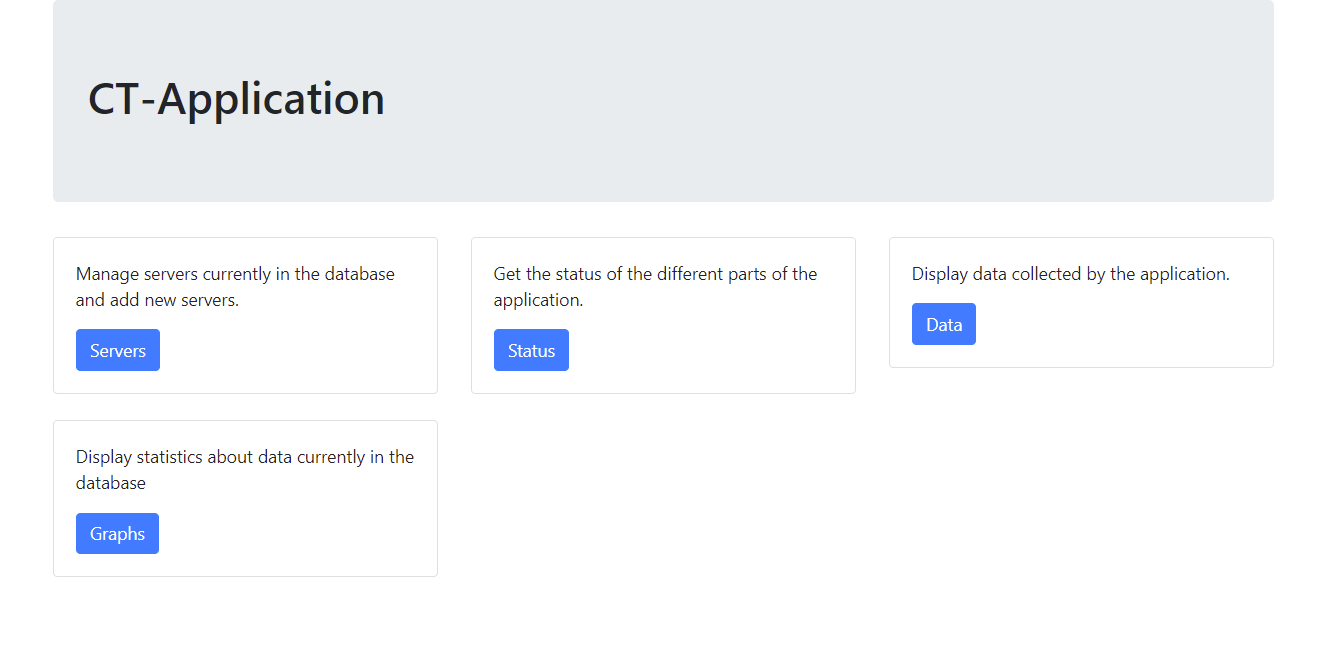
\includegraphics[width=\paperwidth]{img/home.png}}
\caption{Page principale de CT-Application}
\label{home-fig}
\end{figure}

\subsection{Première exécution}

Cette section détaille les étapes à suivre pour ajouter le premier serveur à l'application pour permettre le téléchargement de certificats.

Pour ajouter le premier serveur dans l'application, dirigez vous vers l'onglet \emph{Servers} et créez le serveur en utilisant le formulaire à gauche sur la page, comme présenté dans la figure \ref{add-srv-fig}.

\begin{figure}
\begin{center}
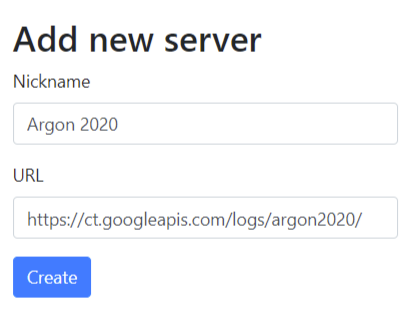
\includegraphics[width=0.5\textwidth]{img/add-srv.png} 
\end{center}
\caption{Ajouter un serveur}
\label{add-srv-fig}
\end{figure}

Pour commencer à télécharger les certificats depuis le nouveau serveur, appuyer sur le bouton \emph{Start} en regard du serveur, comme dans la figure \ref{start-srv-fig}.  Une fois le serveur lancé, l'application va télécharger et filtrer les certificats présents dans les logs du serveur sélectionné.  Plus de détails sur la manière d'afficher les données téléchargées se trouvent dans les sections suivantes.

\begin{figure}
\begin{center}
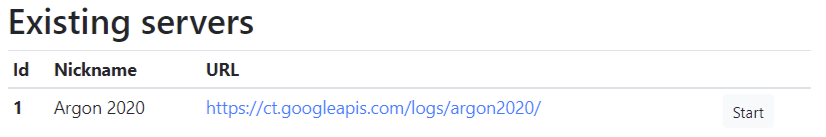
\includegraphics[width=\textwidth]{img/start-server.png} 
\end{center}
\caption{Lancer un serveur}
\label{start-srv-fig}
\end{figure}


\subsection{Gérer les serveurs}

Les serveurs sont la  source de données pour l'application.  Ils peuvent être gérés depuis l'onglet \emph{Servers}.  Cet onglet regroupe tous les serveurs actuellement dans la base de données de l'application et permet d'en ajouter ou de les lancer.

\begin{figure}
\noindent\makebox[\textwidth]{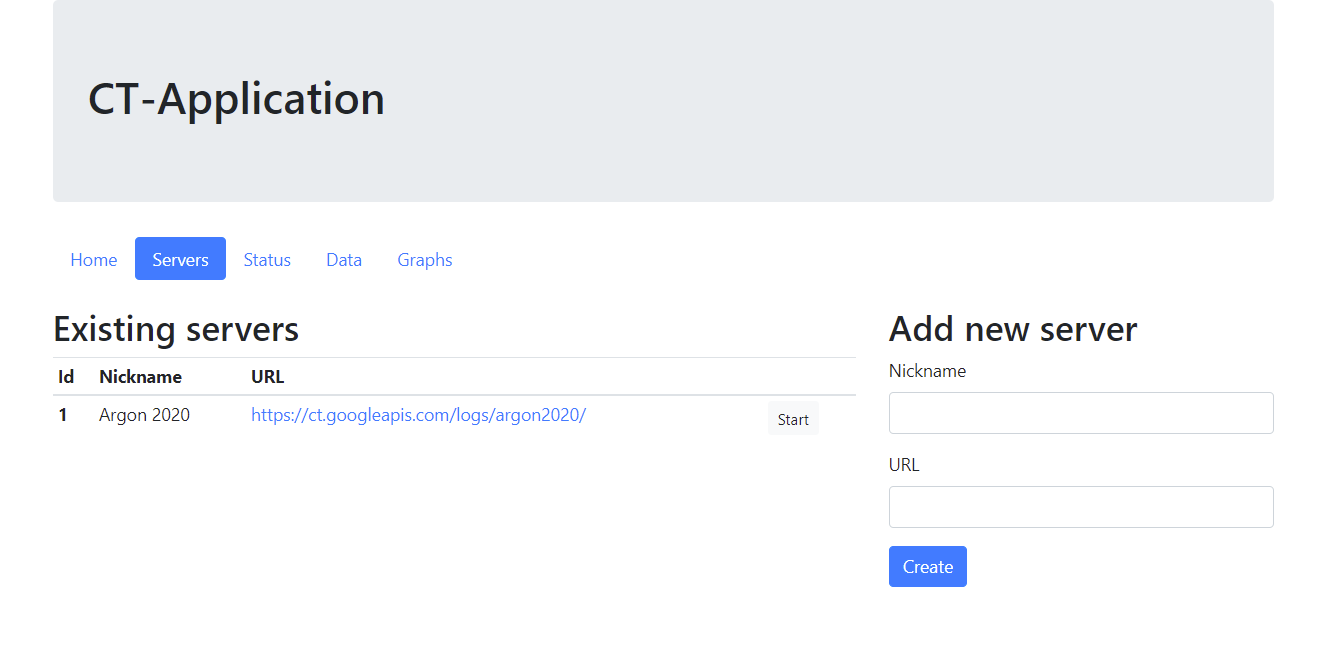
\includegraphics[width=\paperwidth]{img/servers.png}}
\caption{Onglet \emph{Servers}}
\label{servers-fig}
\end{figure}

Pour ajouter un nouveau serveur, choisissez un surnom (\emph{Nickname}) et coller l'\emph{URL}.  Le surnom est facultatif.  Une fois ajouté, le serveur apparaît à la fin de la liste, sur la droite de la page.  Il est nécessaire de lancer le serveur après l'avoir ajouté.  Sinon, rien ne sera téléchargé depuis ce serveur.

Une fois que le bouton \emph{Start} en regard du serveur a été cliqué, tous les logs disponibles sur le serveur au moment du lancement seront téléchargés.  L'application arrêtera ensuite de télécharger des logs à partir de ce serveur.  Pour vérifier si de nouveaux logs sont disponibles sur le serveur, cliquez à nouveau sur \emph{Start}.

Un lien vers l'URL du serveur est fourni dans le tableau.  Certains fournisseurs de logs, comme Cloudflare, affichent un résumé des données présentes sur le serveur à l'adresse pointée par le lien alors que d'autres fournisseurs ne le font pas.

Plus de serveurs peuvent être trouvés sur le site de Certificate Transparency: \url{https://www.certificate-transparency.org/known-logs}.

\subsection{Vérifier le statut}


L'onglet \emph{Status} affiche les informations à propos de l'état actuel des différentes parties du programme.  Une fois qu'un serveur est ajouté dans l'application, le processus d'acquisition des données se divise en quatre étapes.

\begin{description}
\item[Server handling -] Découpe les nouveaux serveurs en tranches pour télécharger les données plus rapidement
\item[Downloader -] Télécharge effectivement les données depuis le serveur
\item[Decoder -] Décode les données téléchargées, conserve uniquement les certificats belges et les enregistre dans la base de données
\item[VAT scrapper -] Tente de retrouver un numéro de TVA sur le site renseigné dans le certificat
\end{description}

Cette division est visible dans l'onglet \emph{Status}.

Depuis cet onglet, il est possible d'arrêter les différentes parties de l'application pour arrêter l'exécution du programme.  A partir de cet onglet, il est également possible de relancer la recherche de numéros de TVA.  Cela s'avère particulièrement utile lorsque l'application a été arrêtée mais que tous les certificats n'ont pas été analysés pour la recherche du numéro de TVA.  Relancer cette recherche aura pour effet de parcourir les sites renseignés dans les certificats qui n'ont pas encore été analysés.

\begin{figure}
\noindent\makebox[\textwidth]{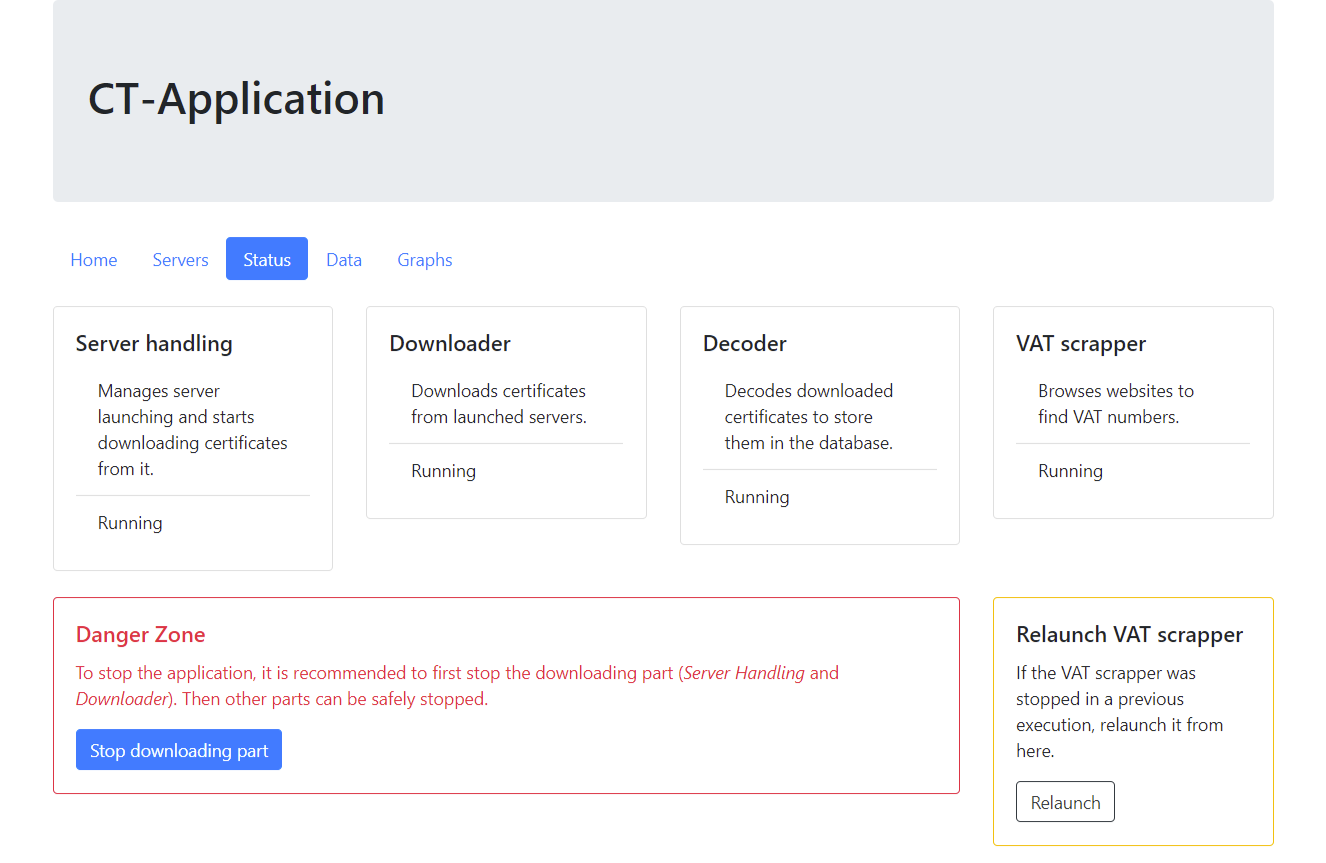
\includegraphics[width=\paperwidth]{img/status.png}}
\caption{Onglet \emph{Status}}
\label{status-fig}
\end{figure}


\subsection{Consulter les données}

L'onglet \emph{Data} affiche les informations relatives aux données collectées depuis les différents serveurs de logs qui ont été ajoutés à l'application.  Cet onglet donne une vue brute des données.  Pour chaque certificat, le sujet, l'émetteur, la période de validité et, s'il a été trouvé, le numéro de TVA sont affichés.

Si, pour un certificat donné, le numéro de TVA a été trouvé, un lien vers la \emph{Banque-Carrefour des Entreprises} est inclus pour permettre d'obtenir plus de détails à propos de l'entreprise.

Le bouton \emph{Only with VAT} permet de basculer entre l'affichage complet et l'affichage des certificats avec un numéro de TVA uniquement.  


\begin{figure}
\noindent\makebox[\textwidth]{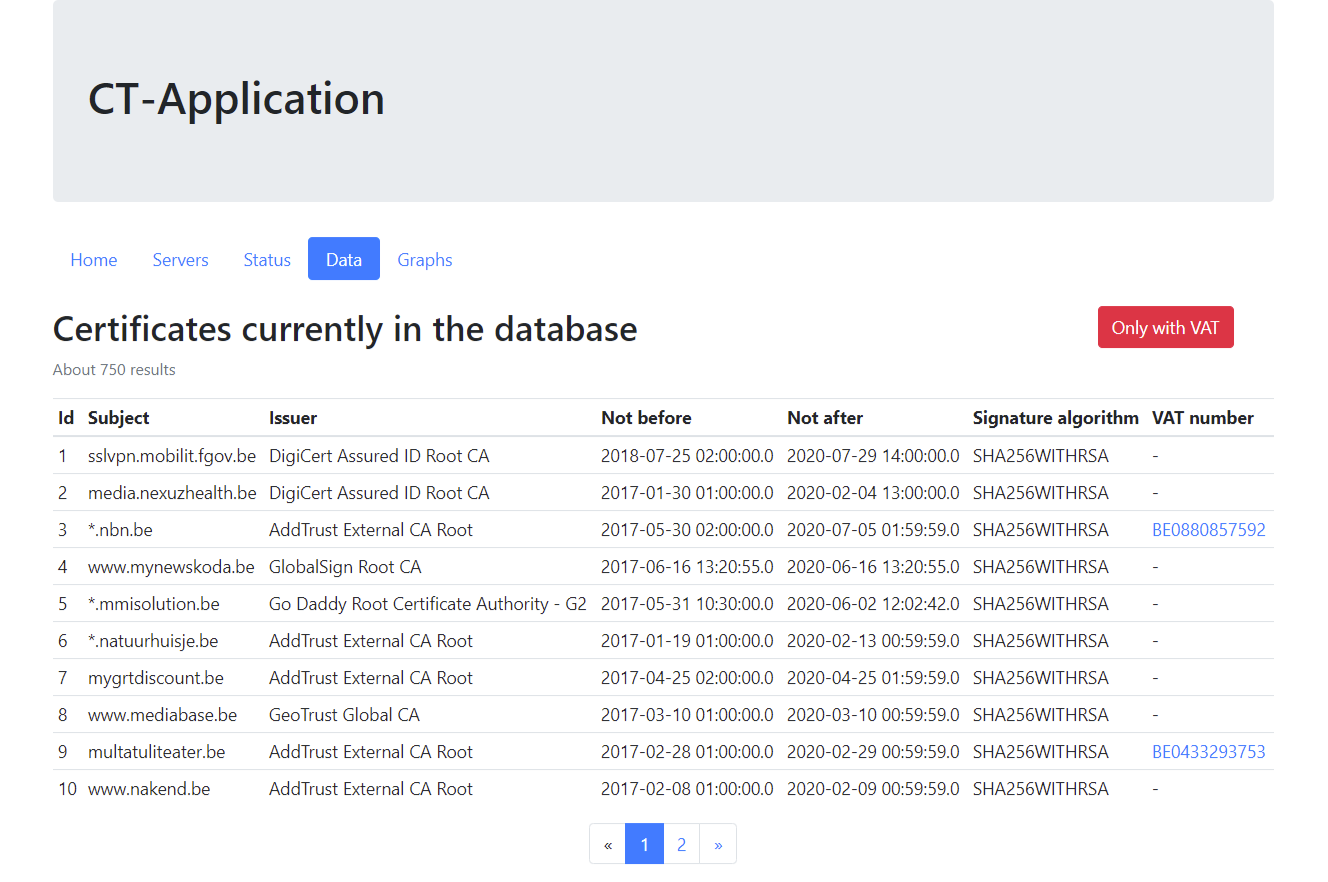
\includegraphics[width=\paperwidth]{img/data.png}}
\caption{Onglet \emph{Data}}
\label{data-fig}
\end{figure}


\subsection{Afficher les graphiques}

L'onglet \emph{Graphs} permet d'afficher un résumé des données actuellement dans la base de données.  Trois graphiques sont disponibles: les émetteurs les plus populaires, les algorithmes de signature les plus populaires et un aperçu de l'état de recherche des numéros de TVA.

\begin{figure}
\noindent\makebox[\textwidth]{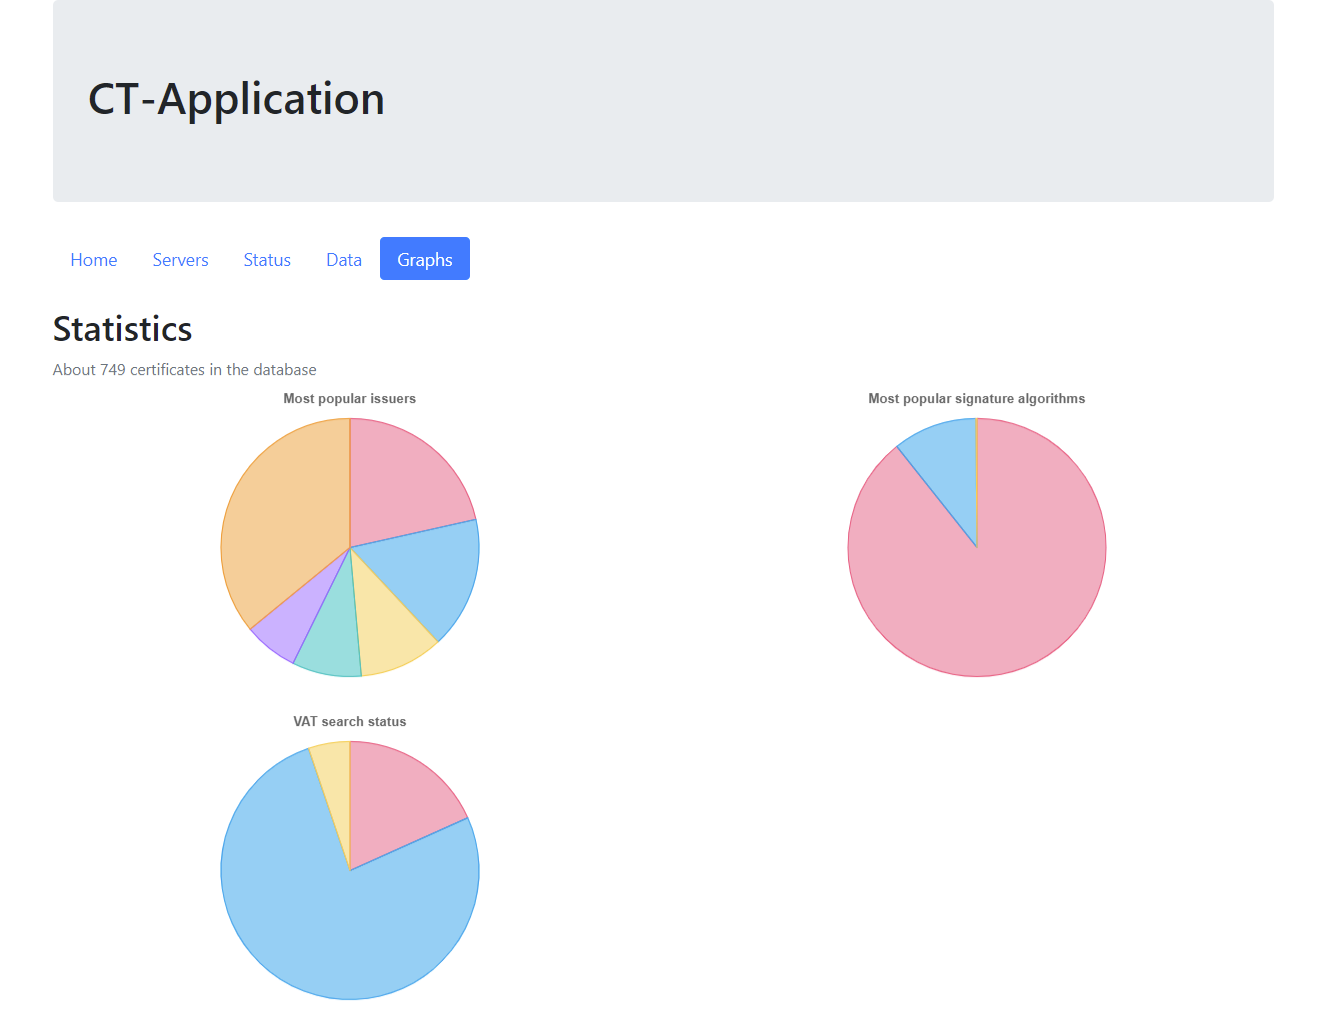
\includegraphics[width=\paperwidth]{img/graphs.png}}
\caption{Onglet \emph{Graphs}}
\label{graphs-fig}
\end{figure}

\clearpage

\section{FAQ}

\subsection{Ma base de données pose problème, comment puis-je y remédier?}

Pour comprendre ce qui pose problème, il est possible d'afficher toutes les requêtes SQL dans le terminal où s'exécute l'application.  Pour activer cette option, arrêtez l'application, modifiez le fichier \path{application.properties} en y ajoutant la ligne ci-dessous et redémarrez l'application.

\begin{minted}{text}
spring.jpa.show-sql=true
\end{minted}

Une fois cette option activée, les requêtes SQL seront affichées dans le terminal et aideront peut-être à identifier la cause du problème.


\subsection{L'application met longtemps à s'arrêter, que puis-je faire?}

Lorsque l'application s'arrête, elle met fin à tous les threads en cours d'exécution et vide la file d'attente des threads.  En fonction du nombre de threads en cours d'exécution, cette opération peut prendre un certain temps.  Attendre l'arrêt de tous les threads et de l'application est la meilleure chose à faire pour éviter une éventuelle corruption des données.

\end{document}
